% !TeX program = lualatex
% !TeX encoding = utf8
% !TeX spellcheck = uk_UA

\documentclass[]{beamer}
\usetheme{PlasmaPhysics}
\usepackage{PlasmaPhysics}
\usetikzlibrary{shadings}

%\NewDocumentCommand{\E}{}{\vec{E}}
%\NewDocumentCommand{\B}{}{\vec{B}}
%\NewDocumentCommand{\J}{}{\vec{j}}
%\NewDocumentCommand{\V}{}{\vec{v}}
%\NewDocumentCommand{\wk}{}{\vec{k}}
%
%\NewDocumentCommand{\divg}{m}{\vec{\nabla}\cdot{#1}}
%\NewDocumentCommand{\rot}{m}{\vec{\nabla}\times{#1}}
%\NewDocumentCommand{\grad}{m}{\vec{\nabla}#1}
%\NewDocumentCommand{\vecdot}{mm}{\left[#1\times#2\right]}
%\NewDocumentCommand{\scdot}{mm}{\left(#1\cdot#2\right)}
%\NewDocumentCommand{\dt}{m}{\frac{\partial #1}{\partial t}}
%\NewDocumentCommand{\ddt}{m}{\frac{\partial^2 #1}{\partial t^2}}

\usepackage{subcaption}
\usepackage{mathtools}
\setlength{\abovedisplayskip}{3pt}
\setlength{\belowdisplayskip}{3pt}
\usetikzlibrary{decorations.pathreplacing}
\newtcolorbox{mysidebyside}[1][]{
    notitle, sidebyside, blanker,
    sidebyside align=center seam,
    halign=center,
    lefthand width=.5\textwidth,
    #1
}



\graphicspath{{pictures/}}
\title[Лекції з фізики плазми]{\bfseries\huge Явища переносу в плазмі}
\subtitle{\bfseries Лекції з фізики плазми}
\author{Пономаренко С. М.}
\date{}
% https://www.youtube.com/watch?v=zv9Y7YmHyBk
\def\stext#1{\text{
        \makebox[0pt]{
            \tikz[baseline] {\node[text width=50pt, align=center, execute at begin node=\setlength{\baselineskip}{-0.5ex}, blue] {#1};}
        }
}}


\begin{document}




%===============================================================================
\usebackgroundtemplate{
	\tikz\node[opacity=0.1]{\includegraphics[width=\paperwidth,height=\paperheight]{background}};%
}


\begin{frame}
	\thispagestyle{empty}
	\titlepage
\end{frame}

% ============================== Слайд ## ===================================
\begin{frame}{Коефіцієнти переносу в газах}{}
	\begin{block}{Коефіцієнт теплопровідності}
		\begin{equation*}
			\chi  = \frac52 \frac{\tau n T}{m}
		\end{equation*}
	\end{block}

	\begin{block}{Коефіцієнт в'язкості}
		\begin{equation*}
			\eta  = n T \tau
		\end{equation*}
	\end{block}
	\begin{block}{Коефіцієнт дифузії}
		\begin{equation*}
			D  = \frac13 \frac{\ell^2}{\tau} = \frac13 v_T^2\tau.
		\end{equation*}
	\end{block}
	\begin{block}{}\justifying
		В формулах $\ell$ --- середня довжина вільного пробігу частинки,\\ $\tau$ --- середній час між зіткненнями.
		\begin{equation*}
			\tau = \frac{\ell}{v_T} = \frac1{n v_T \sigma},
		\end{equation*}
		$\sigma$ --- транспортний переріз кулонівських зіткнень.
	\end{block}
\end{frame}
% ===========================================================================

% ============================== Слайд ## ===================================
\begin{frame}{Кулонівські зіткнення в плазмі}{}
	\begin{onlyenv}<1>
		\begin{block}{}\justifying
			\alert{Пружні зіткнення електронів з іонами зумовлені далекодійними кулонівськими полями} --- електрон взаємодіє одночасно з багатьма
			розсіювальними
			центрами. Переважна більшість таких зіткнень характеризується великими прицільними параметрами і, відповідно, малими кутами розсіювання. В
			результаті \alert{траєкторія електрона набуває вигляду майже гладенької кривої лінії}. Тепер про довжину вільного пробігу можна говорити лише
			умовно.
		\end{block}
		\begin{alertblock}{}\centering
			За довжину вільного пробігу можна вважати ділянку траєкторії електрона, на якій напрямок його швидкості зміниться на $\pi/2$.
		\end{alertblock}
		%---------------------------------------------------------
		\begin{figure}[h!]\centering
			%			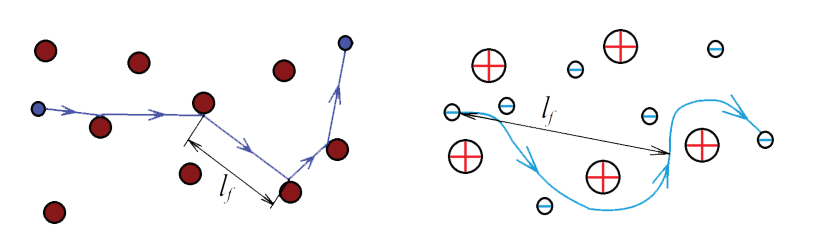
\includegraphics[width=0.75\linewidth]{pictures/elpath}
			\newcommand{\midarrow}{\tikz \draw[-latex] (0,0) -- +(.1,0);}


%---------------------------------------------------------
\begin{minipage}[c]{0.5\linewidth}\centering
    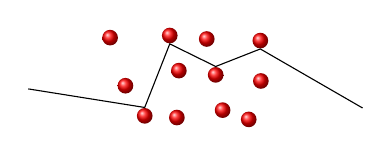
\begin{tikzpicture}[scale=0.5]
    \pgfmathsetseed{3}
    \foreach \x in {1,...,4} {
        \foreach \y in {1,...,3} {
            \node[circle, ball color=red, inner sep=2pt] (\x-\y) at ({\x+rnd}, {\y+0.5*rnd}) {};
        }
    }
\draw (-1, 2) -- node[sloped] {\midarrow} (1-1.north)
-- node[sloped] {\midarrow} (2-3.south)
-- node[sloped] {\midarrow} (3-2.north)
-- node[sloped]
{\midarrow} (4-3.south)
-- node[sloped]
{\midarrow} ++(-30:3);
\end{tikzpicture}
\end{minipage}%
%---------------------------------------------------------
\begin{minipage}[c]{0.5\linewidth}\centering

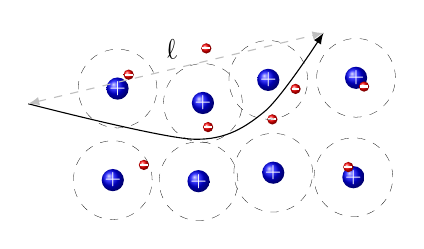
\begin{tikzpicture}[scale=0.5, >=latex,
]
    \pgfmathsetseed{6}
    \foreach \x in {1,...,4} {
        \foreach \y in {1,...,2} {
            \node[circle, ball color=blue, inner sep=0pt, text=white, font=\scriptsize] (\x-\y) at ({2*\x+0.5*rnd}, {2*\y+1*rnd}) {+};
             \draw[dashed, ultra thin] (\x-\y) circle (1);
            \node[circle, ball color=red, inner sep=0pt, text=white, font=\scriptsize] (e-\x-\y) at ({2*\x+1*rnd}, {2*\y+2*rnd}) {\tikz {\draw[thick]
            (0,0) -- ++(0.1,0);} };
        }
    }

%\draw[gray!50, step=1cm] (0, 0) grid[] (10, 6);
\draw[-latex] plot [smooth] coordinates { (0, 4.2) (4.2, 3.3) (6, 4) (7.5, 6) };
\draw[dashed, <->, gray!50] (0, 4.2) -- node[sloped, above, text=black] {$\ell$} (7.5, 6);
\end{tikzpicture}
\end{minipage}
%---------------------------------------------------------


		\end{figure}
		%---------------------------------------------------------
	\end{onlyenv}
	\begin{onlyenv}<1-2>
		\begin{equation*}
			\sigma = \frac{4\pi}{9}\left( \frac{e^2}{T} \right)^2 \ln \Lambda.
		\end{equation*}
	\end{onlyenv}
	%де $\ln\Lambda$ --- кулонівський логарифм.
	\begin{onlyenv}<2>
        \begin{block}{}
    $\ln\Lambda$ --- кулонівський логарифм. Для плазми $\Lambda = \frac{r_D}{b_0} $ являє собою максимальну прицільну відстань, виражену в
    одиницях ${b_0}$ (усереднену за максвеллівським розподілом).
    Величина ${b_0} = \frac{e^2}{mv^2}$ --- величина прицільного параметру, при якому кут відхилення дорівнює $\pi/2$.
    \end{block}
		\begin{center}
			\begin{tblr}{
					colspec={cc},
					vlines,
					hlines,
				}                        & $T$, еВ & $n$, см\textsuperscript{-3} & $\ln\Lambda$ \\
				Лабораторна плазма       & $0.2$   & $10^{11}$                   & $10.2$       \\
				Плазмовий тор            & $100$   & $10^{13}$                   & $13.7$       \\
				Термоядерний реактор     & $10^4$  & $10^{18}$                   & $16.0$       \\
				Плазма лазерного синтезу & $10^3$  & $10^{24}$                   & $6.8$
			\end{tblr}
		\end{center}
	\end{onlyenv}
\end{frame}
% ===========================================================================

% ============================== Слайд ## ===================================
\begin{frame}{Характерні часи релаксації в плазмі}{}
	\framesubtitle<1>{Час електрон-електронної релаксації}
	\begin{onlyenv}<1>
		\begin{equation*}
			\omega_p = \sqrt{\frac{4\pi e^2n}{m_e}}, \quad r_D = \sqrt{\frac{T}{4\pi e^2n_e}}, \quad N_D = \frac{T^{3/2}}{(4\pi)^{1/2}e^3n_e^{1/2}}.
		\end{equation*}
		\begin{block}{}
			\begin{equation*}
				\tau_{ee} = \frac{m^{1/2}T_e^{3/2}}{n_e e^4\ln\Lambda} \sim \frac{N_D}{\omega_p\ln\Lambda}
			\end{equation*}
		\end{block}
	\end{onlyenv}
	\framesubtitle<2>{Час іон-іонної релаксації}
	\begin{onlyenv}<2>
		\begin{equation*}
			\tau_{ii} = \frac{m^{1/2}T^{3/2}}{n_e e^4\ln\Lambda} \sim \frac{N_D}{\omega_p\ln\Lambda} \left(\frac{M_i}{m_e}\right)^{1/2}
			\left(\frac{T_i}{T_e}\right)^{3/2}.
		\end{equation*}
	\end{onlyenv}
	\framesubtitle<3>{Час електрон-іонної релаксації}
	\begin{onlyenv}<3>
		За одне зіткнення електрона з іоном перший передає другому частку своєї енергії порядку $m_e/M_i$. Щоб електрон передав іонам майже всю свою енергію,
		він повинен здійснити порядку $M/m_e$ зіткнень. Тому час електрон-іонної релаксації, тобто час вирівнювання температур електронів та іонів, можна
		оцінити як:
		\begin{equation*}
			\tau_{ei} \approx \tau_{ee}\frac{M}{m} \sim \frac{N_D}{\omega_p\ln\Lambda} \left(\frac{M_i}{m_e}\right) .
		\end{equation*}
	\end{onlyenv}
	\framesubtitle<4>{Порівняння часів релаксації}
	\begin{onlyenv}<4>
		\begin{block}{}\justifying
			\begin{equation*}
				\tau_{ei} \gg \tau_{ii} \gg \tau_{ee}
			\end{equation*}
			У плазмі з помітним відхиленням розподілу частинок за швидкостями від рівноважного спочатку  встановлюється максвеллівський розподіл для
			електронів, потім для іонів, і лише в останню чергу вирівнюються температури електронів та іонів.
			\begin{equation*}
				\ell_e = v_{T_e} \tau_{ee} \sim \frac{T^2}{n_ee^4 \ln\Lambda}, \quad
				\ell_i =  v_{T_i} \tau_{ii} \sim \ell_e \left( \frac{T_i}{T_e} \right)^2 .
			\end{equation*}

			Довжини вільного пробігу електронів та однозарядних іонів в ізотермічній плазмі однакові, оскільки вони не залежать від швидкостей
			частинок і визначаються лише концентраціями та перерізами пружного розсіювання, які для цих частинок однакові.

		\end{block}
	\end{onlyenv}
\end{frame}

% ============================== Слайд ## ===================================
\begin{frame}{Коефіцієнт теплопровідності, в'язкості та електропровідності}{}
	\begin{block}{}\justifying
		\begin{equation*}
			\chi_e \sim \frac{T_e^5}{m_e^{1/2}e^4\ln\Lambda}, \quad \chi_i \sim \frac{T_i^5}{M_i^{1/2}e^4\ln\Lambda}.
		\end{equation*}
		Оскільки звичайно $T_e \gg T_i$, і $M_i \gg m_e$, то $\chi_e \gg \chi_i$ --- \alert{теплопровідність плазми переважно забезпечується
			електронами}.
	\end{block}

	\begin{block}{}\justifying
		\begin{equation*}
			\eta_e \sim \frac{T_e^5m_e^{1/2}}{e^4\ln\Lambda}, \quad \chi_i \sim \frac{T_i^5M_i^{1/2}}{e^4\ln\Lambda}.
		\end{equation*}
		При $T_e = T_i$ маємо $\eta_i \gg \eta_e$,	тобто \alert{в'язкість плазми визначається переважно іонною компонентою}. Ця обставина
		зумовлена тим, що перенесення імпульсу здійснюється переважно іонами.
	\end{block}

	\begin{block}{}\justifying
		\begin{equation*}
			\sigma \sim \frac{T_e^5}{m_e^{1/2} e^2\ln\Lambda}.
		\end{equation*}
		Електропровідність плазми збільшується зі збільшенням температури.
	\end{block}
\end{frame}
% ===========================================================================

% ============================== Слайд ## ===================================
\begin{frame}{Дифузія в плазмі}{}
	\begin{block}{}\justifying
		\begin{equation*}
			D_e = \frac13 \frac{T_e^5}{m_e^{1/2}e^4 n \ln\Lambda}, \quad D_i = D_e \left( \frac{m_e}{M_i} \right)^{1/2} \left(
			\frac{T_i}{T_e}\right)^{5/2}  .
		\end{equation*}
		Електрони (з меншими масами та більшими тепловими швидкостями) дифундують швидше від іонів. Формули справедливі лише за умов локальної
		термодинамічної рівноваги.
	\end{block}
	\begin{block}{}\justifying
		Дифузія плазми, навіть за відсутності магнітного поля --- більш складний процес порівняно з дифузією нейтрального газу.


		\bigskip

		Формули характеризують дифузію електронів лише в початкові моменти часу.  В результаті відбувається розділення зарядів і з’являється електричне
		поле, яке пригальмовує електрони і прискорює іони. За рахунок цього плазма дифундує як єдине ціле. Такий процес називається \alert{амбіполярною
			дифузією}.
	\end{block}
\end{frame}
% ===========================================================================

% ============================== Слайд ## ===================================
\begin{frame}{Амбіполярна дифузія}{}
	\begin{block}{}\justifying
		\alert{Потоки електронів та іонів  у неоднорідній плазмі обумовлюються одночасно} градієнтом її концентрації та електричним полем, обумовленим
		поляризацією плазми, тобто власне \alert{дифузією} і \alert{дрейфом}. Для плазми, градієнт концентрації якої паралельний осі х, можна записати:
		\begin{equation*}
			\Gamma_e = n_e\vec{v}_e = -\mu_e n \vec{E} - D_e\grad{n}, \quad \Gamma_i = n_i\vec{v}_i = \mu_i n \vec{E} - D_i\grad{n}.
			%    \divg{\vec{E}} &= 4\pi (n_i - n_e).
		\end{equation*}

		\begin{onlyenv}<1>
			{\scriptsize Якби виконувалася нерівність $\Gamma_e \neq \Gamma_i$ то в плазмі виник би сильне розділення зарядів, тому слід очікувати, що швидкості
				дифузії іонів і електронів якось підлаштовуватимуться одна до одної, так щоб потоки цих частинок були однакові. }

			\medskip

			\begin{equation*}
				\vec{E} = \frac{D_i - D_e}{\mu_i + \mu_e} \frac{\grad{n}}{n}.
			\end{equation*}
		\end{onlyenv}
		\begin{onlyenv}<1-2>
			Концентраційний потік:
			\begin{equation*}
				\Gamma = - \frac{\mu_iD_e + \mu_eD_i}{\mu_i + \mu_e}\grad{n}.
			\end{equation*}
		\end{onlyenv}
		\begin{onlyenv}<2>
			Це співвідношення являє собою закон Фіка з новим коефіцієнтом
			\begin{equation*}
				D_a  = \frac{\mu_iD_e + \mu_eD_i}{\mu_i + \mu_e}
			\end{equation*}
			який називається \alert{коефіцієнтом амбіполярної дифузії}.
		\end{onlyenv}
		\begin{onlyenv}<3>
			Оскільки ре $\mu_e \gg \mu_a$ то
			\begin{equation*}
				D_a  \approx D_i + \frac{\mu_i}{\mu_e}D_e = D_i + \frac{T_e}{T_i}D_i .
			\end{equation*}
			Для ізотермічної плазми ($T_e = T_i$):
			\begin{equation*}
				D_a \approx 2D_i.
			\end{equation*}
			Через наявність електричного поля, спричиненого поділом зарядів, коефіцієнт дифузії іонів збільшується вдвічі.
		\end{onlyenv}
	\end{block}
\end{frame}
% ===========================================================================

\end{document}

